% !TEX root = main.tex

\section{Our Techniques}\label{sec:techov}
In this section, we provide a high-level overview of our techniques. Both of our results follow a similar high-level rationale, and thus throughout this overview, we mainly focus on the techniques for proving the STB conjecture whenever $B\in O(1)$ (Theorem~\labelcref{thm:MDST_intro}). Towards the end, we describe the additional ideas needed to obtain the result for $SB\ll T$ (Theorem~\labelcref{thm:MDST2_intro}).


Before explaining the ideas, let us describe the challenge more precisely. We are given a compressing function $h:[N]\times [M]\to [N]$, modeled as a random oracle, and we want to upper bound the probability of a non-uniform attacker in finding a collision in an $\MD_h$ instance with a random salt. We model non-uniform attackers by thinking of them as two-stage adversaries $\advA = (\advA_1,\advA_2)$. The offline part $\advA_1$ is unbounded in running time, and its only restriction is that it can output only $S$ bits. This output is the non-uniform advice given to the online part $\advA_2$ which is then allowed to make up to $T$ queries after which it must output a $B$-block collision for $\MD_h$ and terminate. We assume unbounded running time for both parts $\advA_1$ and $\advA_2$ and only restrict the output-size for $\advA_1$ and the number of queries for $\advA_2$. We refer to such a two-stage adversary $(\advA_1,\advA_2)$ as a $(S,T)$-adversary. In the context of length-$B$ collisions in $\MD_h$, the game is as follows:
\begin{itemize}
    \item $\advA_1$ has unbounded access to $h$ and it outputs $\sigma\in \{0,1\}^S$.
    \item  $\advA_2$ gets $\sigma$ as input along with a random salt $a\in [N]$.
    \item $\advA_2$ outputs $\alpha,\alpha'$. 
    \item $\advA$ wins if $\alpha\neq \alpha'$, $\alpha,\alpha'$ consist of $\le B$ blocks, and $\MD_h(a,\alpha)=\MD_h(a,\alpha')$.
\end{itemize}


There are essentially two main generic approaches known in the literature for proving bounds of this sort. The first is the so-called \emph{pre-sampling} technique, originally due to Unruh~\cite{Unruh07}, and the second is a compression argument. The first technique reduces the problem from considering general hash functions and adversaries $(\advA_1,\advA_2)$ as above to a simpler model (and associated attacker) called the \emph{bit-fixing} model. The advantage of the latter model is that it is typically easier to analyze and results in clean proofs. The second technique is based on a simple information-theoretic idea that \emph{random bits cannot be compressed}.\footnote{
Specifically,  it is impossible to save $w$ bits of information about a random string, except with probability $2^{-w}$.} Thus, an attacker that succeeds in finding collisions is used to compress some random information that is used in the game, and thereby contradiction is reached. This technique, while being extremely influential in many fields and problems in computer science (e.g., ``Algorithmic Lov{\'{a}}sz Local Lemma''~\cite{MoserT10}, lower bounds on cryptographic constructions~\cite{GennaroT00,DeTT10,GhoshalT20}, analyzing hardness of problems in the non-uniform setting~\cite{DodisGK17,CorriganGibbsK18}  and time-space tradeoffs for quantum algorithms~\cite{ChungGLQ20}), often results in technical and complex proofs.
 
It would have been convenient if any non-trivial bound on our problem could be obtained using the bit-fixing technique. Unfortunately, Akshima et al.~\cite{AkshimaCDW20} observed that finding short collisions is relatively easy in the {bit-fixing} model. Hence, the only remaining potentially helpful technique is based on compression. Indeed, Akshima et al.~\cite{AkshimaCDW20}, as their primary technical contribution, managed to carry out such an argument for the particular case of $B=2$, and already then their proof is highly non-trivial and consists of a tedious case analysis. We distill some of the main ideas underlying their general framework approach\footnote{We note that~\cite{ChungGLQ20} introduced an equivalent framework in independent work.} next—this will be useful for us, as well.

\heading{The framework.} We reduce the task of handling arbitrary $(S, T)$-adversaries to the problem of handling $(S, T)$-adversaries, where the preprocessing part $\advA_1$ is degenerate and outputs a fixed string $\sigma$, independent of $h$. Specifically, we define a game, parameterized by $u\in \mathbb{N}_{>0}$, where $\advA_2$ has an arbitrary size $S$ string $\sigma$ hard-coded, and its goal is to find a collision relative to a given salt. $\advA_2$ wins the game if it succeeds in finding a collision when executed with \emph{every one} of $u$ uniformly random salts (there is no $\advA_1$ in this game). The reduction shows that if the best possible adversary $\advA_2$ has advantage $\epsilon$ in the modified game, then the best advantage of an $(S, T)$-adversary in the original game is (roughly) $O(\epsilon^{1/u})$ for $u\approx S$. 
This reduction, formalized in Lemma~\labelcref{lem:nu2ai}, is adapted from Akshima et al.~\cite{AkshimaCDW20} and it uses the beautiful ``constructive Chernoff bound'' of Impagliazzo and Kabanets~\cite{AR:ImpKab10}.\footnote{The use of this reduction is the main (and perhaps only) point of similarity between our proof and \cite{AkshimaCDW20}'s.} 

The advantage of considering the new game is that there is no $\advA_1$, so it is easier to handle. But, to obtain a meaningful result for the original $(S, T)$ game, say an upper bound of $\epsilon$, we need to prove a somewhat stronger upper bound for the new game, that is, roughly $\epsilon^{u}$.  This means, in other words, that we need to show how to compress about $\log (1/\epsilon)$ bits \emph{per each one of the $u$ salts}. 
(Actually, keep in mind that it suffices to achieve this on average!) 
For our target~$\epsilon$, we therefore have the following goal.

\begin{center} 
\textbf{Main challenge}: 
For every one of the $u$ salts, we need to ``save/compress'' (on average) roughly the following number of bits:
\begin{align*}
\log\left(\min\left\{\frac{N}{uT(\log u)^{2(B-2)}B^2},\frac{N}{T^2}\right\}\right).
\end{align*}
\end{center}
By impossibility of non-trivial compression, this would imply that $\advA_2$ must succeed with probability at most 
$$\epsilon\le O\left(\left(\frac{uT(\log u)^{2(B-2)}B^2}{N}+\frac{T^2}{N}\right)^u\right)\;,$$
which would give our result when plugged into the framework. 

%We focus on the ideas underlying our proof of the upper bound on the new game.

\heading{The compression argument.} 
The random string that we shall compress consists of the set of salts denoted $U$, as well as the function $h$.
We give encoding and decoding algorithms that use $\advA_2$ first to encode the pair $(U,h) $ and then use the result to fully decode them whenever $\advA_2$ wins the game. If $\advA_2$ wins with good enough probability, the output of the encoding procedure will be non-trivially short with good probability, which is a contradiction. 


\begin{remark}
 Akshima et al.~\cite{AkshimaCDW20} used the same approach for $B=2$, but their proof does not seem to scale for larger values of $B$. Specifically, their proof involves an exhaustive case analysis. It seems like a naive attempt to generalize their bound to larger values of $B$ would proliferate the number of cases needed to be analyzed, making it unmanageable.  One of our key conceptual insights is a structural characterization of collisions in $\MD_h$ that prevents this explosion in the number of cases needed to be handled. While our analysis applies to any $B$, the number of total cases we consider is roughly the same as Akshima et al.
\end{remark}


\heading{A first attempt and a glimpse at the challenge.} 
%To encode $(U,h)$ the main idea is to run $\advA_2$ with the salts in $U$ as input and omit some of the evaluations of $h$, and recover %these omitted evaluations by running $\advA_2$ on the salts of $U$ while decoding. 
%While the strategy is not fully specified, let us first see why it might even be hopeful by making a strong simplifying assumption. 
Let us make a strong (and typically false) assumption: \emph{the adversary $\advA_2$ never repeats any query to $h$ across all the $u$ runs.}\footnote{While we can assume without loss of generality that $\advA_2$ does not repeat queries within a single execution (since it is not memory-bounded), it is not very reasonable to assume that it will never repeat queries across different executions on different salts.} Since we can assume (w.l.o.g) that if $\advA_2$ outputs $(\alpha,\alpha')$ when run on salt $a$, it has queried $h$ at all values needed to compute $\MD_h(a,\alpha)$ and $\MD_h(a,\alpha')$, we are guaranteed that for  each of the salts $u\in U$  there are at least two \emph{distinct} queries which have the same answer, i.e., a collision. The indices of these queries reside in $[T]$ as this is the query complexity of $\advA_2$ when executed on the particular salt $a$. Thus, we could avoid encoding the answer of the second query and instead encode these two indices in $T$ and remove the answer of the second query from evaluations of $h$. This saves us $\log (N/T^2)$ bits for every salt, giving us even more savings than what we are aiming for. Such compression, in turn, would imply that the birthday attack is optimal, no matter what $B$ is (which makes sense given our assumption but is clearly false for general attackers). 

A naive way to get rid of the assumption (that queries never repeat across different $u$ runs) would be to encode the index of the other query among all $uT$ queries made (instead of $T$). 
But, this would eventually result in another multiplicative $S$ term in our bound. Namely, we would only be able to save $\log (N/(ST^2))$ bits per salt which is too little for us (as it leads to a trivial upper bound). This motivates us to look more closely at how MD collisions are formed, what kind of queries could be involved, and how we could leverage the fact that collisions are short to get more efficient encoding.

\heading{The mouse structure and query types.} We consider the graph implicitly formed through the queries made by $\advA_2$ when running on salts $a_1,\ldots,a_u \in U$.
The nodes of the graph are the possible salts and there is a directed edge from salt $a$ to $a'$ with label $\alpha$ if $h(a,\alpha)=a'$ and this query was made by $\advA_2$.
\begin{figure}[t]
    \centering
    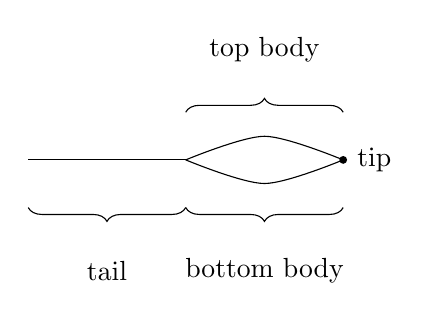
\begin{tikzpicture}
        \draw (-1,0) -- (1,0);
        % \node[circle,inner sep=1pt,fill=red,label=left:{salt}] at (0,0) {};% 
        \node[circle,inner sep=1pt,fill=black,label=right:{tip}] at (3,0) {};% 
        \draw [decorate,decoration={brace,amplitude=5pt,mirror,raise=4ex}]
      (1,0) -- (3,0) node[midway,yshift=-3em]{} 
                          node[midway,yshift=-4em]{bottom body};
      \draw [decorate,decoration={brace,amplitude=5pt,mirror,raise=4ex}]
      (-1,0) -- (1,0) node[midway,yshift=-3em]{}
                            node[midway,yshift=-4em]{tail};
      \draw [decorate,decoration={brace,amplitude=5pt,raise=4ex}]
      (1,0) -- (3,0) node[midway,yshift=3em]{}
                          node[midway,yshift=4em]{top body};
        \draw plot[smooth] coordinates{(1,0) (2,0.3) (3,0)};
        \draw plot[smooth] coordinates{(1,0) (2,-0.3) (3,0)};
    \end{tikzpicture}
    \caption{A mouse structure. For ease of visual representation we do not draw the nodes and edges of the graph, instead represent it as a continuous structure.} \label{fig:mouse-structure-to}
\end{figure}

Suppose that $\advA_2$, when run on salt $a_i$, outputs $(\alpha,\alpha')$. Since $\advA_2$ wins on every salt in $U$, its output on salt $a_i$, denoted $\alpha,\alpha'$ must satisfy: (1) $\MD_h(a_i,\alpha)=\MD_h(a_i,\alpha')$, (2) $\alpha\neq \alpha'$, and (3) $\alpha,\alpha'$ are at most $B$ blocks long. 
Without loss of generality we can assume that the adversary $\advA_2$ outputs a ``minimal" collision, i.e., one that does not contain a prefix which is a collision by itself. For instance, say the collision is $x_1,x_2,x_3,x_4,x_5,x_6$ and $y_1,y_2,y_3,y_4,y_5,y_6$ (wrt salt $a$) and it happens that $x_1,x_2,x_3,x_4$ and $y_1,y_2,y_3,y_4$ already collide (wrt same salt $a$), we can simply ignore $x_5,x_6,y_5,y_6$.
Consider the \emph{core} sub-graph of the query graph that is induced by all the queries made by $\advA_2$ that are \emph{required} to evaluate $\MD_h(a,\alpha)$ and $\MD_h(a,\alpha')$. This sub-graph is what call a \textbf{mouse structure}. Important parts of the mouse structure are the tail, top and bottom body, and the tip,  as depicted in Fig.~\labelcref{fig:mouse-structure-to}.
Our entire approach is based on studying these mouse structures to come up with encoding strategies.  

Given the concept of a mouse structure and our discussion from above about the adversary, possibly repeating queries motivates us to classify each query into one of three types. The first is called \new\ and refers to queries made for the first time. The rest of the queries are called \emph{repeated}, and they are further classified into two types, depending on whether they previously appeared in some mouse structure or not. Specifically, a repeated query is called \frep\ if the same query was already part of the mouse structure for some earlier salt, and otherwise, a repeated query is called \urep. 

Intuitively, we want to save bits when the answer of a \new\ query was the input salt of a repeated query. A \frep\ query whose salt is the answer of a \new\ query facilitates such savings since we can encode the answer to the query by storing its index along with the index of the previous query and the corresponding index within the mouse structure—a total of $\approx \log (uTB)$ bits instead of $\log N$—which eventually turns into an $STB/N$ term in the upper bound, as conjectured. The problem is with encoding \urep\ queries—there seems to be no trivial way to write the index of the previously-made query with less than $\log (uT^2)$ bits, which is too much (since it will eventually turn into a $ST^2/N$ term in the upper bound).




\heading{Some ``easy'' mouse structures.} 
We observe that some cases of mouse structures readily give us a way to have efficient encoding and save sufficiently many bits. We offer three examples to convey intuition on how our analysis is done.
Throughout, let us assume that every mouse structure contains at least one \new\ query—otherwise, we will ignore this mouse structure altogether.\footnote{In the technical section, we refer to salts $a_j$ in $U$ that were not the input salt of a query when running $\advA_2$ on $a_i$ for $i<j$ as \emph{fresh}. It follows that mouse structures for fresh salts will always have a \new\ query. For salts that are not fresh, it is relatively straightforward to achieve some compression by avoiding storing these salts in the encoding of $U$. For now, the reader can imagine that all salts are fresh for simplicity.} 

As a first example, if two $\new$ queries form the tip of the mouse structure of salt $a_j$, we can simply encode the index of these queries within the queries made while handling this salt—this uses $2\log T$ bits instead of $\log N$ bits which is sufficient. As another example, if a self-loop forms the body of the mouse structure and the self loop query is \new\ or \urep\ (this later case happens when a query which has the same answer as its input salt forms the body of the mouse structure, had been made while the adversary was run on some previous salt, but was not part of any earlier mouse structures), we can simply encode the index of the self loop query in the list of queries used to handle this salt and avoid encoding the answer of the query—this uses $\log (uT)$ bits instead of $\log N$ which is again sufficient. As the last example, suppose the answer to a \new\ query is a salt that appeared in some earlier mouse structure. In this case, we can avoid encoding the answer of the \new\ query and instead encode the index of the query and which of the salts in the previous mouse structures is the answer—this uses $\log (2uB)$ bits (because there are at most $2B$ salts in mouse structures and at most $u$ mouse structures) instead of $\log N$ which is also sufficient. 


\heading{Some ``hard'' mouse structures.} The aforementioned easy cases give rise to a relatively easy encoding that results in an optimal $STB/N$ term. Next, we focus on the more complex cases, which cause our bound to have the extra $\approx B\cdot (\log S)^B$ factor.

Assume that there is a mouse structure where there are two salts $a'$ and $a''$ such that $a'$ is the input salt to a \frep\ query, $a''$ is the answer to a \new\ query, and the path from $a''$ to $a'$ in the mouse structure consists of only \urep\ queries (as shown in Figure~\labelcref{fig:hardcaseto}). By definition, the distance between $a'$ and $a''$ is at most $B$.\footnote{By being slightly more careful, we can show that the distance is $B-2$ but we ignore this fact for the overview.} Potential savings could be achieved by not encoding $a''$, the answer of the \new\ query, as it can essentially be extracted from already-observed queries. We can easily encode the appropriate index of the query in the mouse structure and the salt $a'$ using roughly $\log (uB)$ bits, but how can we encode the information about the path back from $a'$ to $a''$?

The non-triviality is that for each node on this path, there might be many possible ways to reach it among all the different queries that have been already made, i.e., if each node on this path has fan-in $m$, namely an $m$-multi-collision, then the natural encoding of the path back would cost at most $\log (m^B)$ bits, specifying which back edge to take for every node. 
Here, $m$ could be very large, e.g., as large as $S$ or even larger, making the whole result meaningless for most reasonable parameters settings. (We also need to encode the length of the path, which would lead to the additional multiplicative $B$ factor, but we ignore it in the discussion here.)
\ovhardcasefig

We get around this problem of $m$ potentially being very large by observing that one of the following two cases holds:
\begin{itemize}
\item \emph{Many small multi-collisions:} either the fan-in of every node along the path (i.e., the number of previously-made queries whose result is a node on this path) is smaller than $\log u$, or
\item \emph{One large multi-collision:} there is (at least one) node on the path where the fan-in is at least $\log u$.
\end{itemize}

In the earlier case, we encode the path back as mentioned above, where we write the index of each back edge. This costs us $B\cdot \log\log u$ bits, which eventually translates to an extra $(\log S)^B$ term,\footnote{Remember that the actual term is $(\log S)^{B-2}$ and that is why the proof of Akshima et al.~\cite{AkshimaCDW20}, in which it was assumed that $B=2$, did not have an extra term that depends on $S$.} as we have in our main theorem. The question is, what do we do when the second case occurs.

The idea is to leverage the fact that there is a large multi-collision and obtain our savings from a completely different place. Specifically,
we remember the index of all the queries involved in the multi-collision and the common answer. A calculation reveals that if the collision consists of $\approx \log u$ edges, we can already save enough. 
One subtlety is that the same multi-collision might repeat throughout many different mouse structures, and we need to make sure not to double count the savings from a single multi-collision more than what we get. The reason why we do not double count is that a single large-enough (i.e.,  with $\log u$ edges) multi-collision saves us enough bits for about $\log u$ different structures, and at the same time, such a multi-collision can appear in at most  $\log u$ mouse structures.\footnote{We mention that multi-collisions in hash functions have been studied on their own right (e.g.,\ifnum\eprintversion=1 ~\cite{Joux04,BermanDRV18,BitanskyKP18,KomargodskiNY18,Dinur20})\else~\cite{Joux04,Dinur20})\fi, but our context is totally different.}

Let us finally remark that while the above description conveys the main idea underlying our compression strategy, it is somewhat simplified and glossed over many technicalities and the complete specification of all possible cases that our full proof covers. We refer to Section~\labelcref{sec:comparg} for full details.


\heading{Proving the STB conjecture for $S\cdot B\ll T$.} The proof of our second upper bound follows the same overall structure. The only difference is, naturally, in the way we encode reverse paths in mouse structures that have nodes corresponding to \urep\ queries between the output $a''$ of a \new\ query and a  node $a'$ corresponding to a $\frep$ query.

In the earlier proof, when we needed to locate the salt $a''$ from salt $a'$, we encoded the number of edges in between and all the edges on the path. Here, we prove a purely graph-theoretic lemma saying that if for salt $a'$ there are more than $\approx u^2$ salts $a''$ such that there are $d>0$ edges on the shortest path back from $a'$ to $a''$ in the query graph, then there must be $t\geq 1$ multi-collisions in the graph, such that the total number of edges involved in the $t$ multi-collisions is at least $\approx u^2$. While the proof of this lemma is a simple inductive argument, it turns out to be extremely helpful for us. Specifically, if there are $t\geq 1$ different multi-collisions such that a total of at least $\approx u^2$ different queries are involved in the $t$ multi-collisions, \emph{we can save enough by only encoding these multi-collisions and nothing else}. To prove this fact, we consider the minimum savings we can get from encoding these $t$ multi-collisions. We show using some elementary calculus that if there are $\approx u^2$ queries involved in $t$ different multi-collisions, the minimum saving is more than the total amount of savings we need.

Equipped with this fact, we split our analysis into the two following scenarios.
\begin{enumerate}
\item  The first is where for each case where we need to encode the location of $a''$ from $a'$ at a distance $d$, there are at most $\approx u^2$ salts -- here we simply encode the index of the ``right'' $a''$ using $\approx \log u^2$ bits. 
\item The other scenario is when for at least one case, there are more than $\approx u^2$ salts. Here we can save enough by encoding the $t$ multi-collisions involving at least $\approx \log u^2$ that the graph-theoretic lemma guarantees us. We get enough savings by only encoding these $t$ multi-collisions.
\end{enumerate}

The $u^2$ term from the first scenario above turns into an additional factor of the form $S^2$ in the final bound. Due to additional technicalities that we glossed over during this overview, we suffer another multiplicative factor $S$ in our bound, which amounts to having an $S^4$ term. Full details appear in Section~\labelcref{sec:secbound}.


